\documentclass{article}
\usepackage{listings}
\usepackage{listings}
\usepackage{color}
\usepackage{graphicx}
\graphicspath{ {./} }
\usepackage[top=1in, bottom=1.25in, left=1.25in, right=1.25in]{geometry}
\definecolor{mygreen}{rgb}{0,0.6,0}
\definecolor{mygray}{rgb}{0.5,0.5,0.5}
\definecolor{mymauve}{rgb}{0.58,0,0.82}
\lstset{ %
	backgroundcolor=\color{white},   % choose the background color; you must add \usepackage{color} or \usepackage{xcolor}; should come as last argument
	basicstyle=\footnotesize,        % the size of the fonts that are used for the code
	breakatwhitespace=false,         % sets if automatic breaks should only happen at whitespace
	breaklines=true,                 % sets automatic line breaking
	captionpos=b,                    % sets the caption-position to bottom
	commentstyle=\color{mygreen},    % comment style
	deletekeywords={...},            % if you want to delete keywords from the given language
	escapeinside={\%*}{*)},          % if you want to add LaTeX within your code
	extendedchars=true,              % lets you use non-ASCII characters; for 8-bits encodings only, does not work with UTF-8
	frame=single,	                   % adds a frame around the code
	keepspaces=true,                 % keeps spaces in text, useful for keeping indentation of code (possibly needs columns=flexible)
	keywordstyle=\color{blue},       % keyword style
	language=Octave,                 % the language of the code
	morekeywords={*,...},            % if you want to add more keywords to the set
	numbers=left,                    % where to put the line-numbers; possible values are (none, left, right)
	numbersep=5pt,                   % how far the line-numbers are from the code
	numberstyle=\tiny\color{mygray}, % the style that is used for the line-numbers
	rulecolor=\color{black},         % if not set, the frame-color may be changed on line-breaks within not-black text (e.g. comments (green here))
	showspaces=false,                % show spaces everywhere adding particular underscores; it overrides 'showstringspaces'
	showstringspaces=false,          % underline spaces within strings only
	showtabs=false,                  % show tabs within strings adding particular underscores
	stepnumber=2,                    % the step between two line-numbers. If it's 1, each line will be numbered
	stringstyle=\color{mymauve},     % string literal style
	tabsize=2,	                   % sets default tabsize to 2 spaces
	title=\lstname                   % show the filename of files included with \lstinputlisting; also try caption instead of title
}
\author{Polykarpos Thomadakis}
\title{Assignment 1 \\
	\large CS834 Introduction to Information Retrieval\\Fall 2017}
\begin{document}
\maketitle
\section*{Question 1.1}
Think up and write down a small number of queries for a web search engine.
Make sure that the queries vary in length (i.e., they are not all one word). Try
to specify exactly what information you are looking for in some of the queries.
Run these queries on two commercial web search engines and compare the top
10 results for each query by doing relevance judgments. Write a report that answers
at least the following questions: What is the precision of the results? What
is the overlap between the results for the two search engines? Is one search engine
clearly better than the other? If so, by how much? How do short queries perform
compared to long queries?

\subsection*{Answer}
Bing and DuckDuckGo were the two search engines that I compared for the purposes of this assignment. I searched for something that I expected to be a bit hard for them to return the best results without enough words. My search was for examples of Message Passing Interface (MPI) code in C language. 
\\The precision is defined as the number of relevant results recalled by the total number of results recalled :
$$ Precision=\frac{Relevant\;results}{Total\;number\;of\;results} $$
The overlap is defined as the number of results that appear in both search engines for the same query:
$$ Overlap = \frac{Results \in  \mathcal{D\cap B}}{Number\;\;of\;results\;per\;search\;engine}$$\\
where $\mathcal{D,B}$ are the sets of results for DuckDuckGo and Bing respectively.\\
\\\underline{Note for DuckDuckGo:} I did not include the result that is an advertisement in my evaluations,since advertisements are usually biased to come up even when they might not be that relevant.\\
\\I started with a one word query, simply MPI:\\
The acronym MPI is used for many different things, so none of the engines did that well with the one-word query.Bing did not return any relevant result at all, as opposed to DuckDuckGo which returned 3.\\
\\As for the overlap, it was zero for the relevant results, however 3 out of the non relevant results are common. I think it is important to note that and also the fact that the top result for both engines was the same.\\
The results can be seen in figure \ref{fig:mpi} and the precision in each case is:

$$Precision_{DuckDuckGo}=\frac{3}{10}=0.3$$
$$Precision_{Bing}=\frac{0}{10}=0$$
$$Overlap_{Relevant} =\frac{0}{10}=0 \qquad Overlap_{total} =\frac{3}{10}=0.3$$
\begin{figure}
	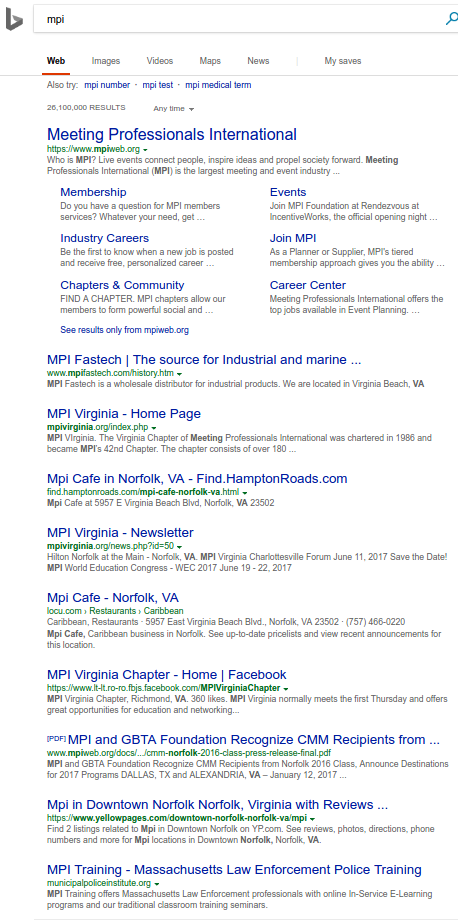
\includegraphics[scale=0.5]{bing_mpi.png}
	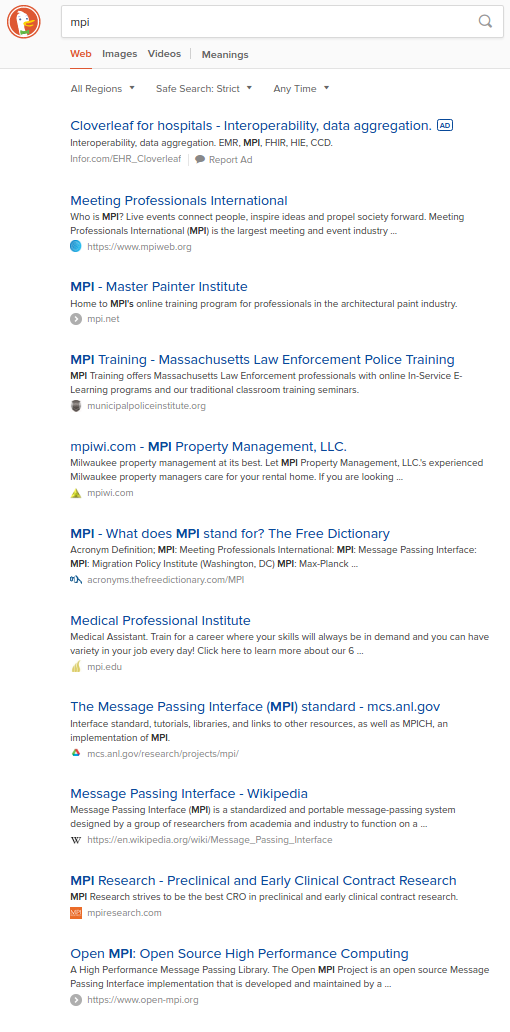
\includegraphics[scale=0.5]{ddg_mpi.png}
	\caption{Comparison of the results for query: MPI}
	\label{fig:mpi}
\end{figure}
\\The next query was with 2 words, MPI C:
\\This time the engines did a much better job.Seven of the results were relevant for DuckDuckGo with the top 4 being relevant and two of the three irrelevants at the last two positions. Bing came short with 6 relevant results, however it made a big difference compared to the previous attempt which had no relevant results. The third, the seventh, the nineth and the tenth results were irrelevant.\\
Six of the relevant results appear in both search engines and nine of the total results are common.\\
The results are presented in figure \ref{fig:mpi_c}.
\begin{figure}
	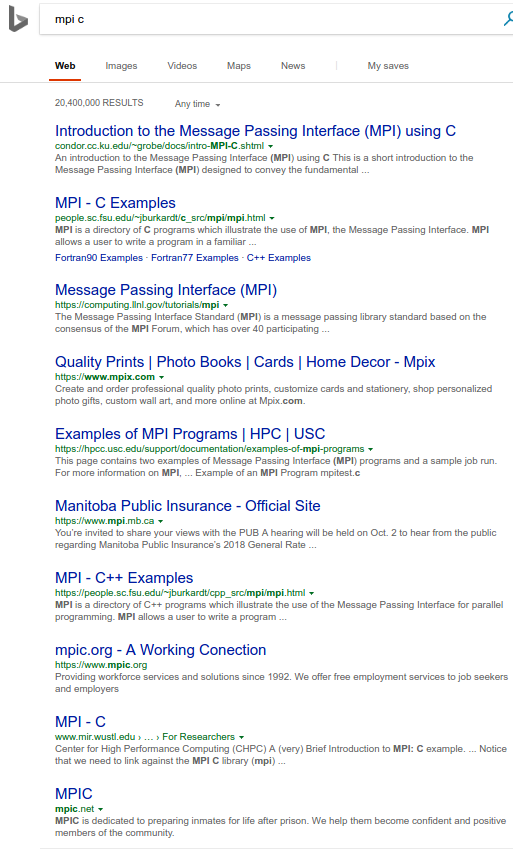
\includegraphics[scale=0.5]{bing_mpi_c.png}
	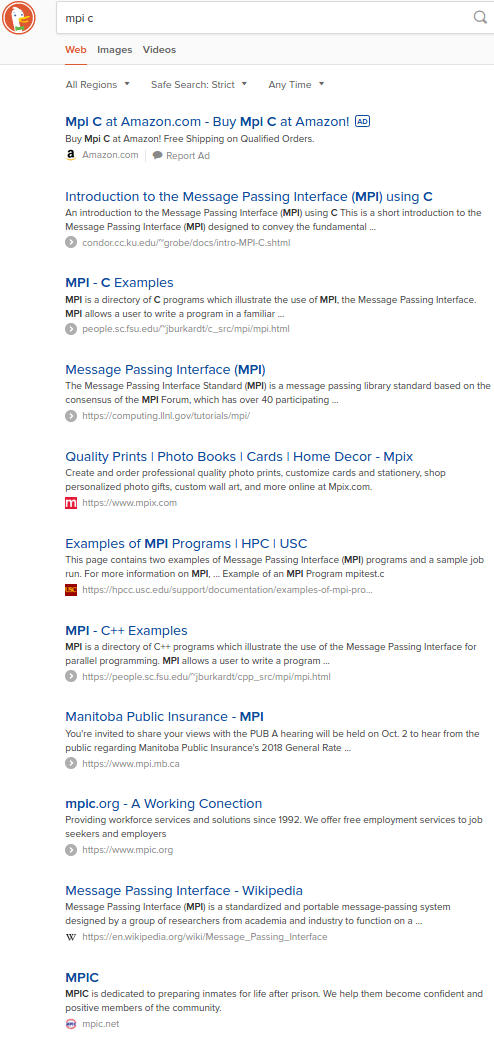
\includegraphics[scale=0.5]{ddg_mpi_c.png}
	\caption{Comparison of the results for query: MPI C}
	\label{fig:mpi_c}
\end{figure}
$$Precision_{DuckDuckGo}=\frac{7}{10}=0.7$$
$$Precision_{Bing}=\frac{6}{10}=0.6$$
$$Overlap_{Relevant} =\frac{6}{10}=0.6 \qquad Overlap_{total} =\frac{9}{10}=0.9$$
\\For the last attempt I used 3 words, MPI C examples:\\
In this case both engines did their best, returning only relevant results. Seven of the results are common for this case with the top two results being in the same ranking order. Another interesting finding is that the total overlap of the two engines has decreased even thought their precision has increased.\\
The results are presented in figure \ref{fig:mpi_c_ex}.
\begin{figure}
	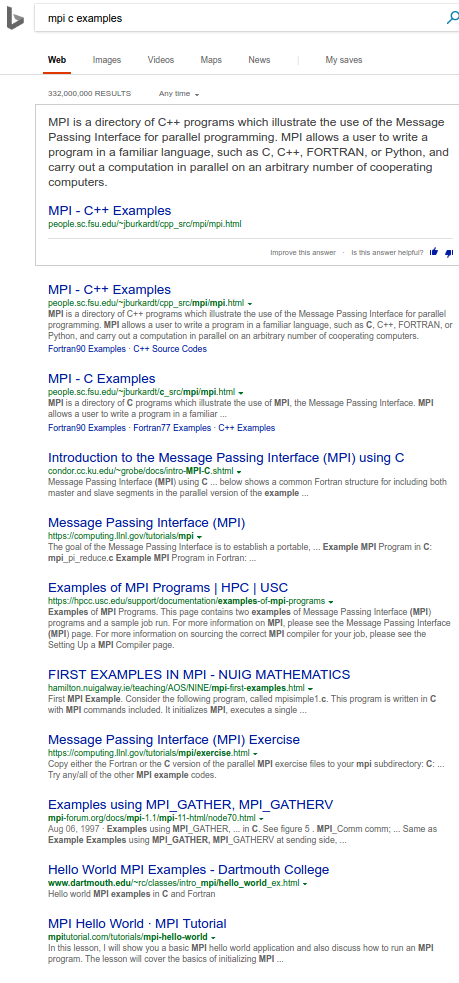
\includegraphics[scale=0.5]{bing_mpi_c_ex.png}
	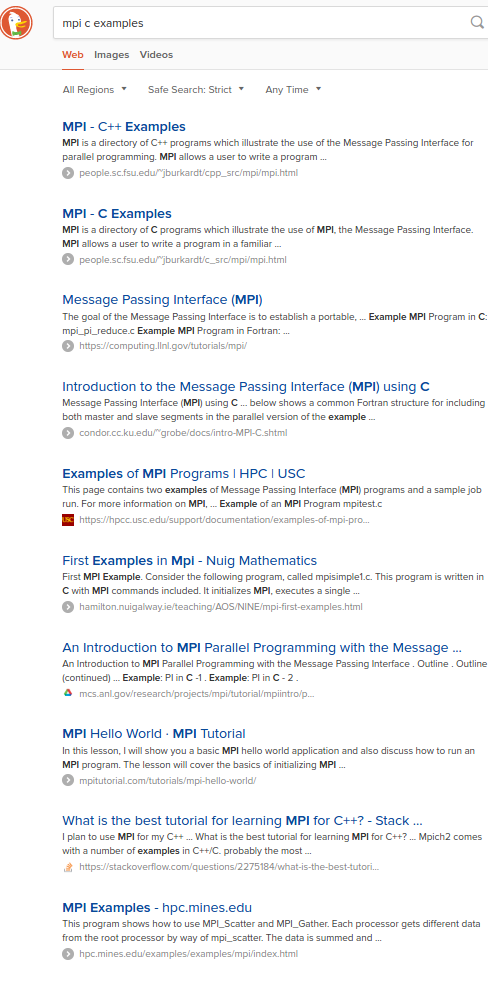
\includegraphics[scale=0.5]{ddg_mpi_c_ex.png}
	\caption{Comparison of the results for query: MPI C examples}
	\label{fig:mpi_c_ex}
\end{figure}
$$Precision_{DuckDuckGo}=\frac{10}{10}=1.0$$
$$Precision_{Bing}=\frac{10}{10}=1.0$$
$$Overlap_{Relevant} =\frac{7}{10}=0.7 \qquad Overlap_{total} =\frac{7}{10}=0.7$$
\\The overall results can be seen in table \ref{tbl:prec_table}. It can be easily noted that the DuckDuckGo search engine outperforms Bing in all cases. In addtion to that, we can see that increasing the length of the query results in a better precision.
\begin{table}[htb]
\centering
\begin{tabular}{|l|l|l|l|l|l|}
\cline{1-5}
&$Prec_{DuckDuckGo}$  &$Prec_{Bing}$  &Relevant Overlap  &Total Overlap  \\ \cline{1-5}
MPI& 0.3 & 0 &  0& 0.3 \\ \cline{1-5}
MPI C& 0.7 & 0.6 &  0.6&0.9  \\ \cline{1-5}
MPI C examples& 1.0 & 1.0 & 0.7 & 0.7 \\ \cline{1-5}
\end{tabular}
\caption{Overall results}
\label{tbl:prec_table}
\end{table}\\
\section*{Question 1.4}
List five web services or sites that you use that appear to use search, not including web search engines. Describe the role of search for that service. Also describe
whether the search is based on a database or grep style of matching, or if the search
is using some type of ranking.
\subsection*{Answer}
Here are five sites that I use that appear to use search:
\begin{enumerate}
	\item \textbf{imdb.com}\\
	The Internet Movie Database (abbreviated IMDb) is an online database of information related to films, television programs and video games, including cast, production crew, fictional characters, biographies, plot summaries, trivia and reviews. The user uses a search query to get information about movies, series or games that are relevant. The search looks to be done against a database.
	\item \textbf{stackoverflow.com}\\
	Stack Overflow is a website featuring questions and answers on a wide range of topics in computer programming. The website serves as a platform for users to ask and answer questions, and, through membership and active participation, to upvote or downvote questions and answers based on their content. This site seems to use a grep style search and also features ranking based on the upvotes of the relevant posts.
	\item \textbf{play.google.com}\\
	Google Play is a digital distribution service. It serves as the official app store for the Android operating system, allowing users to browse and download applications developed with the Android software development kit (SDK) and published through Google. Google Play also serves as a digital media store, offering music, magazines, books, movies, and television programs. Google Play seems to use a database search and using ranking based on the popularity of the results and their user provided reviews.
	\item \textbf{craigslist.com}\\
	Craigslist is a classified advertisements website with sections devoted to jobs, housing, personals, for sale, items wanted, services, community, gigs, resumes, and discussion forums. A user can choose a section and make a search for results relevant to it. The site seems to be using a database search style.
	\item \textbf{github.com}\\
	GitHub is a web-based Git or version control repository and Internet hosting service. It is mostly used for code. It offers all of the distributed version control and source code management (SCM) functionality of Git as well as adding its own features. It provides access control and several collaboration features such as bug tracking, feature requests, task management, and wikis for every project. Github seems to use a database style of search and offers optional ranking based on best match, highest rating, freshness, most forked.
	
\end{enumerate}
\section*{Question 3.7}
Write a program that can create a valid sitemap based on the contents of a directory on your computer’s hard disk. Assume that the files are accessible from a website at the URL http://www.example.com. For instance, if there is a file in your directory called homework.pdf , this would be available at http://www.example.com/homework.pdf . Use the real modification date on the file as the last modified time in the sitemap, and to help estimate the change frequency.
\subsection*{Answer}
The program discovers all the files in the directory given from the user as a command line argument. Then it continues with the files and subdirectories of its subdirectories and goes on until all the files and directories under the given directory have been discovered recursively. To achieve this I use the os.walk() function from the os directory. \\For each file found an xml url structure is generated where the location is registered and then the last modification date information is retrieved with the os.stat() function and is included in the url structure of the file.\\ 
\\Once all files in the tree under the origin directory have been discovered the procedure ends and the xml file is generated with the appropriate format and the structures generated are written on it. \\The user can specify the path where the file will be created, the default location is the current directory.
The source code used can be seen in listing \ref{lst:sitemap} and the sitemap generated for the directory of the assignment can be found in listing \ref{lst:sitemap_out}.\\
\lstinputlisting[language=Python,caption={Sitemap generator},label={lst:sitemap}]{smapgen.py}
\lstinputlisting[language=XML,caption={Generated sitemap},label={lst:sitemap_out}]{sitemap.xml}
\section*{Question 3.9}
Write a simple single-threaded web crawler. Starting from a single input URL
(perhaps a professor’s web page), the crawler should download a page and then
wait at least five seconds before downloading the next page. Your program should
find other pages to crawl by parsing link tags found in previously crawled documents.
\subsection*{Answer}
The crawler starts with one page on its list, the one provided by the user or the default. When all links of the page have been found, the list is filled with the new pages to be crawled. The crawler continues crawling pages in this list, parsing their links.
\\Once all of the pages in the list have been parsed it will continue with their respective links and so on. In order to keep the running time reasonable the user can set the depth in which this procedure will continue crawling. The default depth is 2.\\
\\To avoid downloading big irrelevant files, the crawler will skip non-HTML files by checking the content-type in the header. Command line arguments can be used to set the path where the crawler will create a directory and store the downloaded files.
\\The source code for the crawler is presented in listing \ref{lst:crawler} and a sample of the output for depth 2 can be seen in listing \ref{lst:crawler_output}.\\
\lstinputlisting[language=Python,caption={Web crawler},label={lst:crawler}]{crawl.py}

\lstinputlisting[label={lst:crawler_output},caption={Web crawler sample output}]{sample_output}

\section*{Question 3.12}
Design a compression algorithm that compresses HTML tags. Your algorithm
should detect tags in an HTML file and replace them with a code of your
own design that is smaller than the tag itself. Write an encoder and decoder program.
\subsection*{Answer}
To create the compression algorithm I introduced a 1-1 mapping between each html tag and my compressed tags. HTML tags with 3 or more letters are compressed to 2-3 at most. I start by loading the HTML file and finding all HTML tags in it using regular expressions to match them. Once a tag is matched it will be checked for transformation using the mapping introduced. 
\\For the decompression algorithm I follow the same procedure, but now I perform the mapping the reverse way i.e map the custom tags to the original ones and transform them when needed. 
\\The user must specify an input and output file name for both programs. Of course the output file should not exist, or it will be overwritten.The source code for both programs is found in listings \ref{lst:comp} and \ref{lst:decomp} respectively. Sample input, output can be found in listings \ref{lst:wiki_orig} and \ref{lst:wiki_comp}.
Also the full files are available on my github repository but are not included here because of their size.\\
\lstinputlisting[language=Python,label={lst:comp},caption={Compress source}]{compress.py}
\lstinputlisting[language=Python,label={lst:decomp},caption={Decompress source}]{decompress.py}

\lstinputlisting[language=HTML,linerange=1-30,label={lst:wiki_orig},caption={Sample of the original Wikipedia source file}]{Wiki.html}
\lstinputlisting[language=HTML,linerange=1-30,label={lst:wiki_comp},caption={Sample of the compressed Wikipedia source file}]{Wc.html}

\end{document}